\section{Введение}

\textbf{Цель работы:}
изучение петель гистерезиса ферромагнитных материалов с помощью осциллографа.

\textbf{Оборудование:}
автотрансформатор, понижающий трансформатор, амперметр и вольтметр (мультиметры), резистор, делитель напряжения, интегрирующая
цепочка, электронный осциллогра, тороидальные образцы с двумя обмотками.

\subsection{Теоретическое введение}

\begin{wrapfigure}{l}{0.6\textwidth}
    \centering
    \vspace{-20pt}
        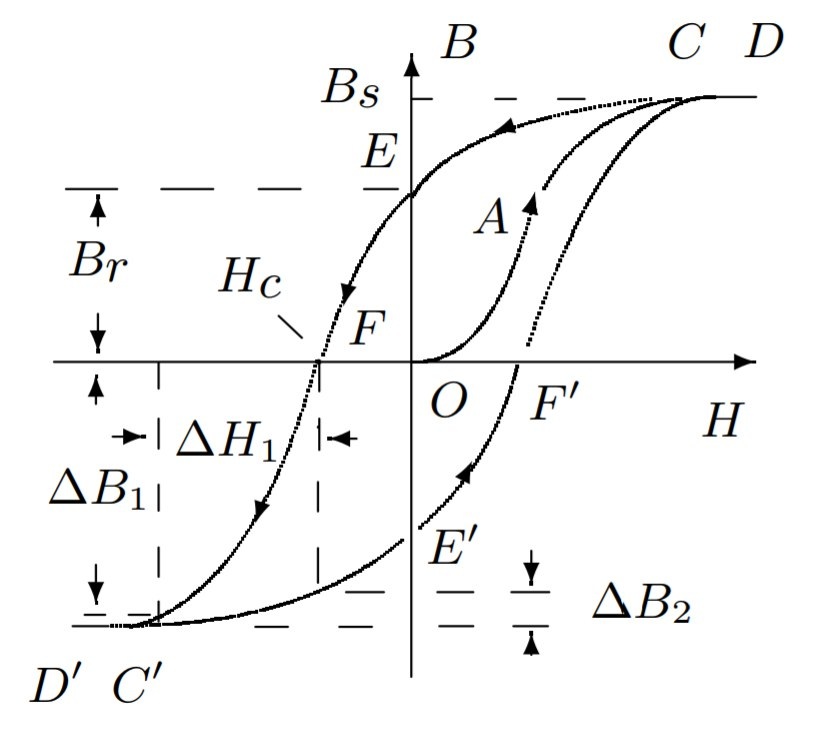
\includegraphics[width=0.7\linewidth]{gist3.jpg}
        \label{fig:sdfsafd}
    \vspace{-10pt}
    \caption{Петля гистерезиса ферромагнетика}
\end{wrapfigure}

Магнитная индукция $\vec{B}$ и напряженность магнитного поля
$\vec{H}$ в ферромагнитном материале неоднозначно связаны
между собой: индукция зависит не только от напряженности, но
и от предыстории образца. Связь между индукцией
и напряженностью поля типичного ферромагнетика иллюстрирует рис. 1. Если
к размагниченному образцу начинают прикладывать магнитное поле, то его намагничивание следует кривой $ OACD $, выходящей
из начала
координат. Эту кривую называют \textit{основной кривой намагничивания}.


Индукция $\vec{B}$ в образце состоит из индукции, связанной с намагничивающим полем
$\vec{B}$, и индукции, создаваемой самим намагниченным
образцом.
В системе СИ эта связь имеет вид

$$\vec{B} = \mu_{0}(\vec{H}+\vec{M}),$$

где $\vec{M}$- \textit{намагниченность} - магнитный момент единичного объема образца, а $\mu_{0}$ - магнитная постоянная.

Намагнитим образец до насыщения - до точки D. Соответствующее
значение индукции $B_{s}$ называют индукцией насыщения. При уменьшении поля $H$ до нуля зависимость $B(H)$ имеет вид кривой $DCE$, и при нулевом поле индукция имеет конечное ненулевое значение. Это остаточная индукция $B_{r}$ . Чтобы размагнитить образец, то есть перевести его в состояние
$F$, необходимо приложить "обратное" магнитное
поле $H_{c}$, которое называют коэрцитивной силой.

Замкнутая кривая $DEFD'E'F'D$, возникающая при циклическом
перемагничивании образца, намагниченного до насыщения, называется \textit{предельной петлей гистерезиса.}


\subsection{Измерение магнитной индукции в образцах.}
Магнитную индукцию удобно определять с помощью ЭДС, возникающей при изменении магнитного потока Ф в катушке, намотанной на образец:

$$\varepsilon = -\frac{d\Phi}{dt}.$$

Тогда отсюда и из формулы $\Phi=BSN_\text{и}$ получаем:
    $$|B|=\dfrac{1}{SN_\text{и}}\int Edt.$$
Для интегрирования сигнала применяют интегрирующие схемы (рис. 2).

    \begin{wrapfigure}{l}{0.6\textwidth}
    \centering
    \vspace{-20pt}
        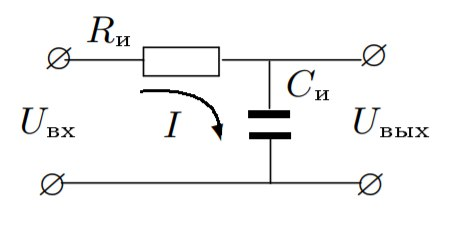
\includegraphics[width=0.7\linewidth]{gist2.jpg}
    \label{fig:sdfsafd}
    \vspace{-10pt}
    \caption{Интегрирующая RC-цепь}
\end{wrapfigure}

Если выходной сигнал намного меньше входного ($U_\text{вых}\ll U_\text{вх},$) ток в цепи пропорционален входному напряжению: $I\simeq\dfrac{U_\text{вх}}{R}$, а напряжение на емкости С

$$U_\text{вых} \approx \frac{1}{RC} \int U_\text{вх}dt$$

Этот вывод тем ближе к истине, чем больше постоянная $\tau=RC$ превосходит характерное время процесса (например, его период). Для синусоидальных напряжений

$$U_\text{вых} = \frac{U_\text{вх}}{RC\Omega},$$

где $\Omega$ - частота сигнала.

В итоге, обозначив параметры интегрирующей цепи через $R_\text{и}$ и $C_\text{и}$, получаем

$$ |B| = \frac{1}{SN_\text{и}} \int U_\text{вх}dt = \frac{R_\text{и}C_\text{и}}{SN_\text{и}}U_\text{вых}$$

\subsection{Экспериментальная установка.}
Схема экспериментальной установки показана на рис. 3.

Действующее значение переменного тока в обмотке N0 измеряется амперметром А (мультиметром GDM). Последовательно с амперметром включено сопротивление $R_{0}$, напряжение с которого подается на вход X электронного осциллографа (ЭО). Это напряжение пропорционально току в обмотке $N_{0}$, а следовательно и напряженности H магнитного поля в образце.

Для измерения магнитной индукции B с измерительной обмотки $N_\text{И}$ на вход интегрирующей RC -цепочки подается напряжение $U_\text{И}$ (UВХ), пропорциональное производной $\dot{B}$, а с выхода снимается напряжение $U_\text{C}$($U_\text{ВЫХ}$), пропорциональное
величине B , и подается на вход Y осциллограа.
Замкнутая кривая, возникающая на экране, воспроизводит в некотором масштабе (различном для осей X и Y ) петлю гистерезиса. Чтобы придать этой кривой количественный смысл, необходимо установить масштабы изображения, т.е. провести калибровку каналов X и Y ЭО. Для этого, во-первых, надо узнать, каким напряжениям (или токам) соответствуют амплитуды сигналов, видимых на экране, и во-вторых,  каким значениям B и H соответствуют эти напряжения
(или токи).

\begin{figure}[h!]
    \centering
    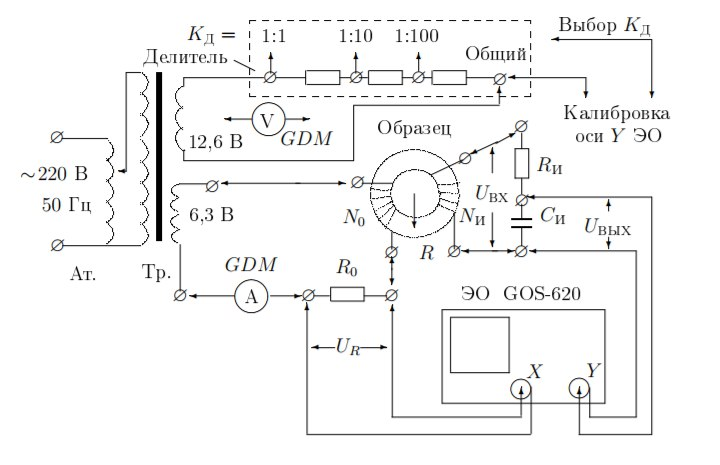
\includegraphics[width=\linewidth]{gist.jpg}
    \caption{Схема установки для исследования намагничивания образцов}
    \label{fig:Holl2}
\end{figure}
